\subsection{Párování na množinách}

\df Systém různých reprezentantů (SRR) {\it množinového systému $(X,S)$ je
prostá funkce $f:S\rightarrow X$ tž. $\forall A \in S: f(A) \in A$.}

\vt (spočetná Hallova) {\it Buď $(X,S)$ množinový systém obsahující spočetně mnoho konečných množin. Pak $(X,S)$ má SRR právě tehdy, když pro libovolný podsystém $T \subseteq S$ s konečně mnoha podmnožinami platí $|\bigcup T| \ge |T|$} (Hallova podmínka)

\dk {\it (v sekci \ref{nekonecna-kombinatorika:hall})}

\subsection{Párování v grafech}

\df Párování je množina hran $M$ taková, že žádné dvě hrany nesdílí společný
vrchol. {\it Perfektní párování} je takové párování, které je incidentní se
všemi vrcholy grafu.

\tv Maximální párování na bipartitním grafu lze nalézt pomocí toků v sítích v
čase $\O(|E| \cdot |M|)$.

\vt Maximální párování v obecném grafu lze nalézt pomocí Edmondsova algoritmu v
čase $\O(|V|^2|E|)$.

\df Vylepšující cesta je cesta, která začíná i končí hranou z $G$, která není v
párování $M$, a na cestě se střídají hrany z $M$ a $E\setminus M$.

\vt (Berge) Párování je maximální právě tehdy, pokud neexistuje vylepšující
cesta.

\alg (Edmondsův květinkový) Algoritmus v každá iterace nalezne zlepšující cestu
a zvětší párování, pokud větší existuje. Díky předchozí větě pokud algoritmus
nenalezne zlepšující cestu, víme, že vydá maximální párování. Zlepšující cesta
se hledá následujícím způsobem:

\begin{enumerate}
	\item Najdi nespárované vrcholy a prohlaš je za kořeny stromů v lese.
	\item Pro každý vrchol přidej do stromu jeho sousedy tak, že na 1. patře je
	pouze kořen, všechny hrany z kořene jsou z $E \setminus M$ a všechny cesty
	od kořene k listům jsou střídavé. Po každém přidání zkontroluj:
	\begin{enumerate}
		\item Vytvořil se lichý cyklus? Pokud ano, kontrahuj ho a pokračuj.
		\item Vede z aktuálního vrcholu hrana do jiného stromu taková, že lze
		vytvořit vylepšující cestu? Pokud ano, vydej tuto cestu.
	\end{enumerate}
	\item Pokud nelze přidat další vrchol, vydej dosavadní párování jako
	maximální.
\end{enumerate}

Algoritmus tedy buduje stromy, pro které cesta kořen-kořen je zlepšující. Liché
cykly se kontrahují, protože bez nich je těžké poznat, zda se nalezla zlepšující
cesta (viz obrázek \ref{blossoms}, kde modrá hrana vytvoří květinku a až po
jejím přidání je možné použít červenou hranu na vylepšující cestu; kotrakce
zjednoduší uvažování cyklů).

Kontrakce nerobijí existenci střídavých cest, protože každá střídavá cesta musí
vést přes stonek, tedy od propojení směrem ke kořeni (jenom v kořeni jsou
vrcholy, kterými lze střídavou cestu ukončit) a každá střídavá cesta si může
vybrat, zda první krok v květince udělá po spárované nebo nespárované hraně.

Vylepšujících cest je najevýš $|E| = m$ po celou dobu běhu algoritmu, jedno
prohledávání spotřebuje nanejvýš $n^2$ času (práce na každém vrcholu může být až
$n$, protože je potřeba potenciálně prohledat hodně sousedů). Celkový běh
algoritmu je tedy $\O(n^2m)$. \qed

\begin{figure}[h!]
	\centering
	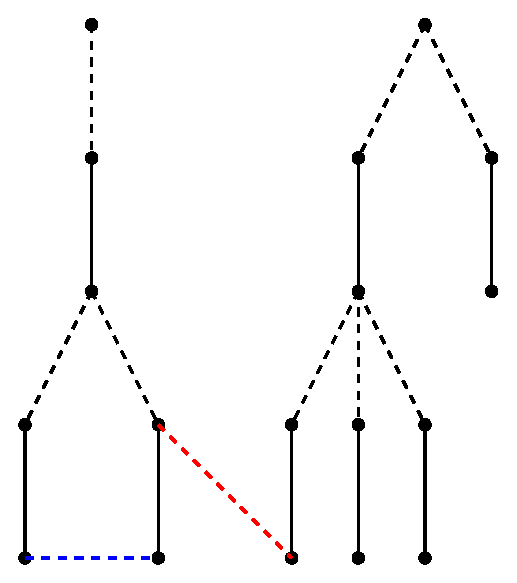
\includegraphics{img/blossoms.eps}
	\caption{Tvorba cyklů a vylepšujících cest v květinkovém algoritmu}
	\label{blossoms}
\end{figure}

\subsection{Otázka velikosti maximálního párování}

\vt (König) Velikost maximálního párování bipartitního grafu odpovídá velikosti
minimálního vrcholového pokrytí.

\vt (Hall) Bipartitní graf $G$ má perfektní párování právě tehdy, když pro každé
$X \subseteq V$ je počet izolovaných vrcholů $G \setminus X$ nanejvýš $X$.

\vt (Tutte) Graf $G$ má perfektní párování právě tehdy, když pro každé $X
\subseteq V$ je počet lichých komponent $G \setminus X$ nanejvýš $|X|$.

\vt (Petersen) Každý 3-regulární graf bez mostů má perfektní párování.

\dk Ukážeme, že každá $X$ splňuje Tutteho podmínku. Označme $q(G \setminus X)$
počet lichých komponent $G \setminus X$. Nechť máme libovolnou $X$ a nějakou
lichou komponentu $C$ (pokud taková neexistuje, podmínka je splněna
automaticky).  Komponenta $C$ má lichý počet vrcholů, ale sudý součet stupňů
(jako každý graf), do grafu ale přispívá celkově lichým součtem stupňů (má lichý
počet vrcholů, každý 3 hrany) -- počet hran spojující $C$ se zbytkem grafu je
tedy lichý, a navíc alespoň $3$, protože jedna hrana by tvořila most. Tedy počet
hran vedoucích z $X$ je alespoň $3q(G \setminus X)$, ale taktéž nanejvýš $3|X|$,
což je maximální počet hran v $S$ z $3$-regularity. Máme tedy $3q(G \setminus X)
\leq\delta X \leq 3|X|$, což po vykrácení $3$ dává Tutteho podmínku a věta je
dokázána. \qed


\subsection{Matching polytope}

Párování stálo u základů polyedrální kombinatoriky, a tak je vhodné zmínit
polytopy, které problém řeší:

\df Označme $\delta(v)$ množinu hran incidentních s vrcholem $v$, $x(e)$ jako
proměnnou pro hranu $e$ a $x(\delta(v)) := \sum_{e \in\delta(v)} x(e)$.

\tv Pro bipartitní graf je Matching polytope následující:
\begin{align}
	x(\delta(v)) \leq 1  & \quad  \forall v \in V \\
	x(e) \geq 0 & \quad \forall e  \in E
\end{align}

Takový polytop (překvapivě) má vždy celočíselné optimální řešení, ale může se
stát, že získáme neceločíselné a přesto optimální (například čtyřcyklus
ohodnocený 1/4). O to horší by byl výsledek tohoto polytopu u nebipartitních
grafů, protože na lichém cyklu získáme lepší neceločíselné, než nejlepší
celočíselné řešení; viz obrázek \ref{matching-polytope}.

Ukazuje se však, že protože matice incidence pro bipartitní graf je totálně
unimodulární, všechna řešení nalezená simplexovým algoritmem jsou celočíselná.

\df Matice $A$ je totálně unimodulární, pokud determinant každé její čtvercové
podmatice je $-1, 0$ nebo $1$.

\df Pokud je $Ax \leq b$ lineární program a $A$ je totálně unimodulární, jsou
všechny vrcholy daného polyedru celočíselné.

\begin{figure}[h!]
	\centering
	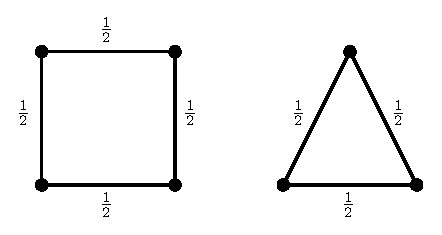
\includegraphics{img/matching-polytope.eps}
	\caption{Ukázka nevhodných neceločíselných řešení}
	\label{matching-polytope}
\end{figure}

\tv Pro libovolný graf je Matching polytope pro perfektní párování následující:
\begin{align}
	x(\delta(v)) \leq 1  & \quad  \forall v \in V \\
	x(e) \geq 0 & \quad \forall e  \in E \\
	x(\delta(U)) \geq 1 & \quad \forall U \subseteq V, |U| \geq 3 \text{ liché
velikosti}
\end{align}

\tv Pro libovolný graf je Matching polytope pro maximální párování následující:
\begin{align}
	x(\delta(v)) \leq 1  & \quad  \forall v \in V \\
	x(e) \geq 0 & \quad \forall e  \in E \\
	x(E[U]) \leq {|U|-1 \over 2} & \quad \forall U \subseteq V, |U| \text{ liché
velikosti}
\end{align}
